\section{Zufallsvariablen}

Zufallsvariablen dienen dazu von einen gegebenen Ereignisraum $(\Omega, \ereignisF)$ zu einem Modellausschnitt $\Omega', \ereignisF'$ überzugehen. 
Es handelt sich also um Abbildungen $\abb{X}{\Omega}{\Omega'}$.
Damit wir auch jedem Ereignis in $\ereignisF'$ eine Wahrscheinlichkeit zuordnen können, benötigen wir	
\begin{equation*}
    A' \in \ereignisF' \follows X^{-1} A' \in \ereignisF		
\end{equation*}
d.h. $X$ sollte \begriff{messbar} sein.

\begin{definition}[Zufallsvariable]
    Seien $(\Omega, \ereignisF)$ und $(\Omega', \ereignisF')$ Ereignisräume. Dann heißt jede messbare Abbildung
    \begin{equation*}
        \abb{X}{\Omega}{\Omega'}
    \end{equation*}
    \begriff{Zufallsvariable} (von $(\Omega, \ereignisF)$) nach $(\Omega', \ereignisF')$/ auf $(\Omega', \ereignisF')$ oder \begriff{Zufallselement}.
\end{definition}

\begin{beispiel}
    \begin{enumerate}[leftmargin=*]
        \item Ist $\Omega$ abzählbar und $\ereignisF = \pows\Omega$, so ist jede Abbildung $\abb{X}{\Omega}{\Omega'}$ messbar und damit eine Zufallsvariable.
        \item Ist $\Omega \subset \Rn$ und $\ereignisF = \borel\Omega$, so ist jede stetige Funktion $\abb{X}{\Omega}{\R}$ messbar und damit eine Zufallsvariable.
    \end{enumerate}
\end{beispiel}

\begin{satz}
    Sei $(\Omega, \ereignisF, \P)$ ein \WRaum und $X$ eine Zufallsvariable von $(\Omega, \ereignisF)$ nach $(\Omega', \ereignisF')$. Dann definiert
    \begin{equation*}
    \P'(A') \defeq \P\left(X^{-1}(A')\right) = \P\left(\set{X \in A'}\right), \quad A' \in \ereignisF'
    \end{equation*}
    ein Wahrscheinlichkeitsmaß auf $(\Omega', \ereignisF')$, welches wir als \begriff{Wahrscheinlichkeitsverteilung von $X$ unter $\P$} bezeichnen.
\end{satz}

\begin{proof}
    Aufgrund der Messbarkeit von $X$ ist die Definition sinnvoll. Zudem gelten
    \begin{equation*}
        \P'(\Omega') = \P(X^{-1}(\Omega')) = \P(\Omega) = 1
    \end{equation*}
    und für $A_1', A_2', \dots \in \ereignisF'$ paarweise disjunkt.
    \begin{equation*}
    \begin{aligned}
        \P' \left( \bigcup_{i \geq 1} A_i' \right) 
        = \P \left(X^{-1}\left( \bigcup_{i \geq 1} A_i' \right) \right) 
        &= \P \left( \bigcup_{i \geq 1} X^{-1}(A_i') \right) \\
        &= \sum_{1 \geq 1} \P(X^{-1} A_i') \quad \text{ da auch } X^{-1}A_1', X^{-1}A_2', \dots \text{ paarweise disjunkt sind} \\
        &= \sum_{1 \geq 1} \P'(A_i)
    \end{aligned}
    \end{equation*}
    Also ist $\P'$ ein Wahrscheinlichkeitsmaß.
\end{proof}

\begin{*bemerkung}
    \begin{itemize}[leftmargin=*, nolistsep]
        \item Aus Gründen der Lesbarkeit schreiben wir in der Folge
        \begin{equation*}
        	\P (X \in A) = \P ( \menge{\omega \colon X(\omega) \in A} )
        \end{equation*}
        \item Ist $X = \id$, so fallen die Begriffe \WMass und \WVerteilung zusammen.
        \item In der (weiterführenden) Literatur zur \WTheorie wird oft auf die Angabe eines zugrundeliegenden Wahrscheinlichkeitsraumes verzichtet und stattdessen eine ``Zufalsvariable mit Verteilung $\P$ auf $\Omega$'' eingeführt.
        Gemeint ist (fast) immer $X$ als Identität auf $(\Omega, \ereignisF, \P)$ mit $\ereignisF = \pows\Omega$ oder $\ereignisF = \borel\Omega$.
        \item Für die Verteilung von $X$ unter $\P$ schreibe $\P_X$ und $X \sim \P_{X}$ für die Tatsache, dass $X$ gemäß $\P_X$ verteilt ist.
    \end{itemize}
\end{*bemerkung}

\begin{definition}
    Zwei Zufallsvariablen sind \begriff{identisch verteilt}, wenn sie dieselbe Verteilung haben.
\end{definition}

Von besonderen Interesse sind für uns die Zufallsvariablen, die nach $(\R, \borel\R)$ abbilden, sogenannte \begriff{reelle Zufallsvariablen}.

Da die halboffenen Intervalle $\borel\R$ erzeugen, ist die Verteilung einer reellen Zufallsvariable durch die Werte $(-\infty, c]$, $c \in \R$ eindeutig festgelegt.

\begin{definition}[Verteilungsfunktion] \label{def: 1.16_verteilungsfunktion}
    Sei $(\R, \borel\R, \P)$ ein \WRaum, so heißt
    \begin{equation*}
        \abb{F}{\R}{[0,1]} \text{ mit } x \mapsto \P((-\infty, x))
    \end{equation*}
    \begriff{(kumulative) Verteilungsfunktion von $\P$}.    
    Ist $X$ eine reelle Zufallsvariable auf beliebigen WRaum $(\Omega, \ereignisF, \P)$, so heißt
    \begin{equation*}
        \abb{F}{\R}{[0,1]} \text{ mit } x \mapsto \P(X \leq x) = \P(X \in (-\infty, x])
    \end{equation*} % TODO everything good with the X's here?
    die (kumulative) Verteilungsfunktion von $X$.
\end{definition}

\begin{beispiel}
    $(\R, \borel\R,\P)$ mit $\P$ Exponentialverteilung mit Parameter $\lambda > 0$
    \begin{equation*}
    \P(A) = \int_{A \cap [0,\infty)}\lambda e^{-\lambda x} \dx \quad A \in \borel\R
    \end{equation*}
    Dann ist
    \begin{equation*}
    F(x) = \P((-\infty, x)) = 
    \begin{cases}
        0 &x \le 0\\
        \int_{0}^{x} \lambda e^{-\lambda y} \dy = 1 - e^{-\lambda x} &x > 0
    \end{cases}\notag
    \end{equation*}
\end{beispiel}

\begin{center}
    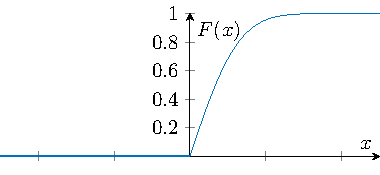
\includegraphics{./stoch_abbildungen/exponentialverteilung_verteilungsfunktion.pdf}
    \captionof{figure}{Verteilungsfunktion der Exponentialverteilung}
\end{center}

\begin{beispiel}
    Das Würfeln mit einem fairen, sechseitigen Würfel kann mittels einer reellen Zufallsvariablen
    \begin{equation*}
        \abb{X}{\menge{1,2,\dots, 6}}{\R} \mit x \mapsto x
    \end{equation*}
    modelliert werden. \\
    Es folgt als Verteilungsfunktion
    \begin{equation*}
	    F(x) 
	    = \P'(X \leq x) = \P(X^{-1}(-\infty,x]) = \P((-\infty,x])
	    = \frac{1}{6} \, \sum_{i=1}^{6} \one_{\menge{i \leq x}}
    \end{equation*}
\end{beispiel}

\begin{center}
    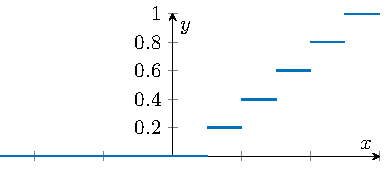
\includegraphics{./stoch_abbildungen/wuerfel_verteilungsfunktion.pdf}
    \captionof{figure}{Verteilungsfunktion des Würfelexperiments}
\end{center}

Diese Erkenntnisse lassen sich auch verallgemeinern:

\begin{satz}
    Ist $\P$ ein \WMass auf $(\R, \borel\R)$ und $F$ die zugehörige Verteilungsfunktion, so gelten
    \begin{enumerate}[nolistsep, topsep=-\parskip]
        \item $F$ ist monoton wachsend
        \item $F$ ist rechtsseitig stetig
        \item $\lim_{x\to -\infty} F(x) = 0$ und $\lim_{x\to \infty} F(x) = 1$
    \end{enumerate}
    Umgekehrt existiert zu jeder Funktion $\abb{F}{\R}{[0,1]}$ mit Eigenschaften (1) bis (3) eine reelle Zufallsvariable auf $((0,1), \borel{(0,1)}, \Uni((0,1)))$ mit Verteilungsfunktion $F$.
\end{satz}

\begin{proof}
    Ist $F$ Verteilungsfunktion, so folgt mit \ref{satz: 1.4_rechenregeln}
    \begin{equation*}
        x \leq y \follows F(x) = \P((-\infty,x]) \overset{\ref{satz: 1.4_rechenregeln}.3}{\leq} \P((-\infty,y]) = F(y)
    \end{equation*}
    und
    \begin{equation*}
        \lim_{m \searrow c} F(x) = \lim_{m \searrow c} \P((-\infty, x]) \overset{\sigma\text{-Stetigkeit}}{=} \P((-\infty, c]) = F(c)
    \end{equation*}
    sowie
    \begin{equation*}
        \lim_{x\to -\infty} F(x) \overset{\ref{satz: 1.4_rechenregeln}.5}{=} \P(\emptyset) \overset{\ref{satz: 1.4_rechenregeln}.1}{=} 0 \quad \und \quad
        \lim_{x\to \infty} F(x) \overset{\ref{satz: 1.4_rechenregeln}.5}{=} \P(\R) = 1
    \end{equation*}
    Umgekehrt wähle
    \begin{equation*}
        X(u) \defeq \inf \menge{x \in \R \colon F(x) \geq u}, \quad u \in (0,1)\\
    \end{equation*}
    Dann ist $X$ eine ``linkseitige Inverse'' von $F$ (auch \begriff{Quantilfunktion} oder \begriff{verallgemeinerte Inverse}).
    Wegen (3) gilt $-\infty < X(u) < \infty$ und zudem
    \begin{equation*}
        \menge{X \leq x} = (0, F(x)) \cap (0,1) \in \borel{(0,1)}
    \end{equation*}
    Da diese halboffene Mengen ein Erzeugendensystem von $\borel\R$ bilden, folgt bereits die Messbarkeit von $X$, also ist $X$ eine \ZV. Insbesondere hat die Menge $\menge{X \le x}$ gerade \person{Lebesgue}-Maß $F(x)$ und damit hat $X$ die Verteilungsfunktion $F$.
\end{proof}

\begin{korollar}
    Ist $\P$ \WMass auf $(\R, \borel\R)$ und $F$ die zugehörige Verteilungsfunktion. Dann besitzt $\P$ genau eine Dichtefunktion $\rho$, wenn $F$ stetig differenzierbar ist, denn dann gilt
    \begin{equation*}
        F(x) = \int_{0}^{x} \rho(x) \dx \quad \text{ bzw } \quad \rho(x) = F'(x)
    \end{equation*}
\end{korollar}

\begin{proof}
    Folgt aus \cref{satz: 1.8_mass_mit_dichte}, der \cref{def: 1.16_verteilungsfunktion} der Verteilungsfunktion und dem Eindeutigkeitssatz \labelcref{satz: 1.9_eindeutigkeitssatz}.
\end{proof}